\documentclass{article}
%==============================================================================%
%	                          Packages                                     %
%==============================================================================%
% Packages
\usepackage[utf8]{inputenc}
\usepackage{graphicx}
\usepackage{amsmath}
\usepackage{amssymb}
\usepackage{braket}
\usepackage[margin=0.7in]{geometry}
\usepackage[version=4]{mhchem}
\usepackage{float}
%==============================================================================%
%                           User-Defined Commands                              %
%==============================================================================%
% User-Defined Commands
\newcommand{\be}{\begin{equation}}
\newcommand{\ee}{\end{equation}}
\newcommand{\benum}{\begin{enumerate}}
\newcommand{\eenum}{\end{enumerate}}
\newcommand{\pd}{\partial}
\newcommand{\dg}{\dagger}
%==============================================================================%
%                             Title Information                                %
%==============================================================================%
\title{Chem237: Lecture 5}
\date{4/11/18}
\author{Shane Flynn,Moises Romero}
%==============================================================================%
%	Everyone Please Make Comments if Something Needs to be Reviewed        %
%                           Or just fix it yourself!                           %
%==============================================================================%
\begin{document}
\maketitle
\section*{Integrals Continued}
%==============================================================================%
\section*{Complex Calculus }
Complex Calculus is a large field (typically a year) we will highlight some useful integration techniques using the complex plane. 

\subsection*{Analytic Function}
Consider the 2D complex plane. 
%==============================================================================%
%%%%%%%%%%%%%%%%%%%%%%%%%%%%%%%%%%%%%%%%%%%%%%%%%%%%%%%%%%%%%%%%%%%%%%%%%%%%%%%%
% We need a 'professional' version of this figure
%%%%%%%%%%%%%%%%%%%%%%%%%%%%%%%%%%%%%%%%%%%%%%%%%%%%%%%%%%%%%%%%%%%%%%%%%%%%%%%%
%==============================================================================%
\begin{figure}[h]
  \centering
  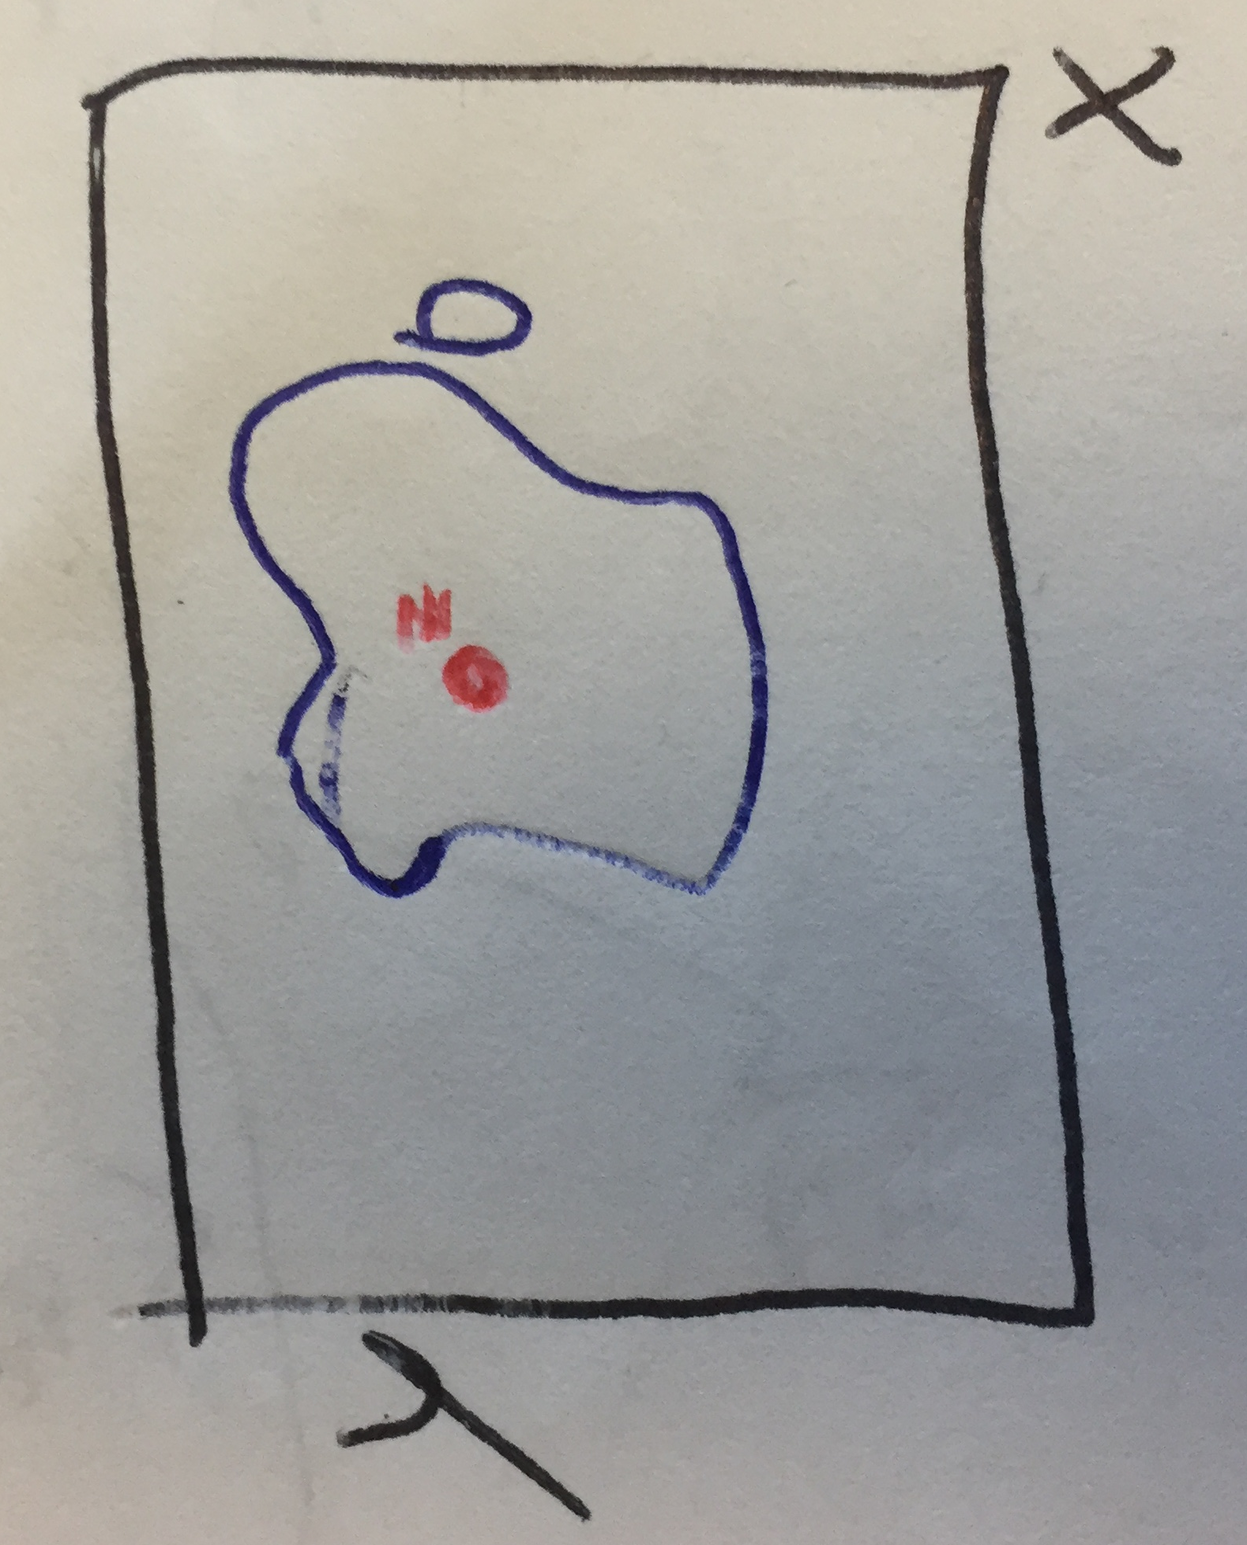
\includegraphics[scale=0.2]{Figures/complex.png}
    \caption{Make a caption (z=x+iy,D=domain(2D))}
  \label{fig:under_damped}
\end{figure}
An \textbf{Analytic Function} in domain (D) if it has derivative for any Z within D.
\be
f'(z) = \lim_{|h|\to 0} \frac{f(z+h)-f(z)}{h}
\ee
%%%%%%%%%%%%%%%%%%%%%%%%Edit this more%%%%%%%%%%%%%%%%%%%%%%%%%%%%%%%%%%%%%%%%%%%%%%%
Where both h,z are $\in \mathbb{C}$. This is a more suddle definition, because h is in complex, no matter how we approach z we will get the same value and the defivitive of the function therefore exists. Weill need to look into this more, vlas says h in complex is a non-trivial definition. 
The takeaway is that an analytic function is important because the derivitive is the same no matter how you approach the limit. 

f(z) is \textbf{Regular} in D if it is analytic and single valued in D.

Examples of non-single valued functions are square roots
$f(z) = \sqrt{z}$ and logarithm functions $f(z)=\ln{(1+z)}$

\subsection*{Cauchy Riemann equations}
In general you can think of complex functions as two different a real and complex component. 
The Cauchy-Riemann equations are used to check if a complex function is analytic (sometimes referred to as holomorphic), in other words if it is differentiable.
It is often useful to define complex functions into their real and complex parts as follows :
\be
f(z) = u(x,y) + iv(x,y)
\ee
Consider h=h$_x$+ih$_y$
\be
\frac{\pd f}{\pd x} = \frac{\pd u}{\pd x} + i \frac{\pd V}{\pd x}
\ee
In general a partial derivitive is just one way to define
\be
f'(z) = \lim_{|h|\to 0} \frac{f(z+h)-f(z)}{h}
\ee
But there are other paths we could take to apprach the derivitive. 
\begin{figure}[h]
  \centering
  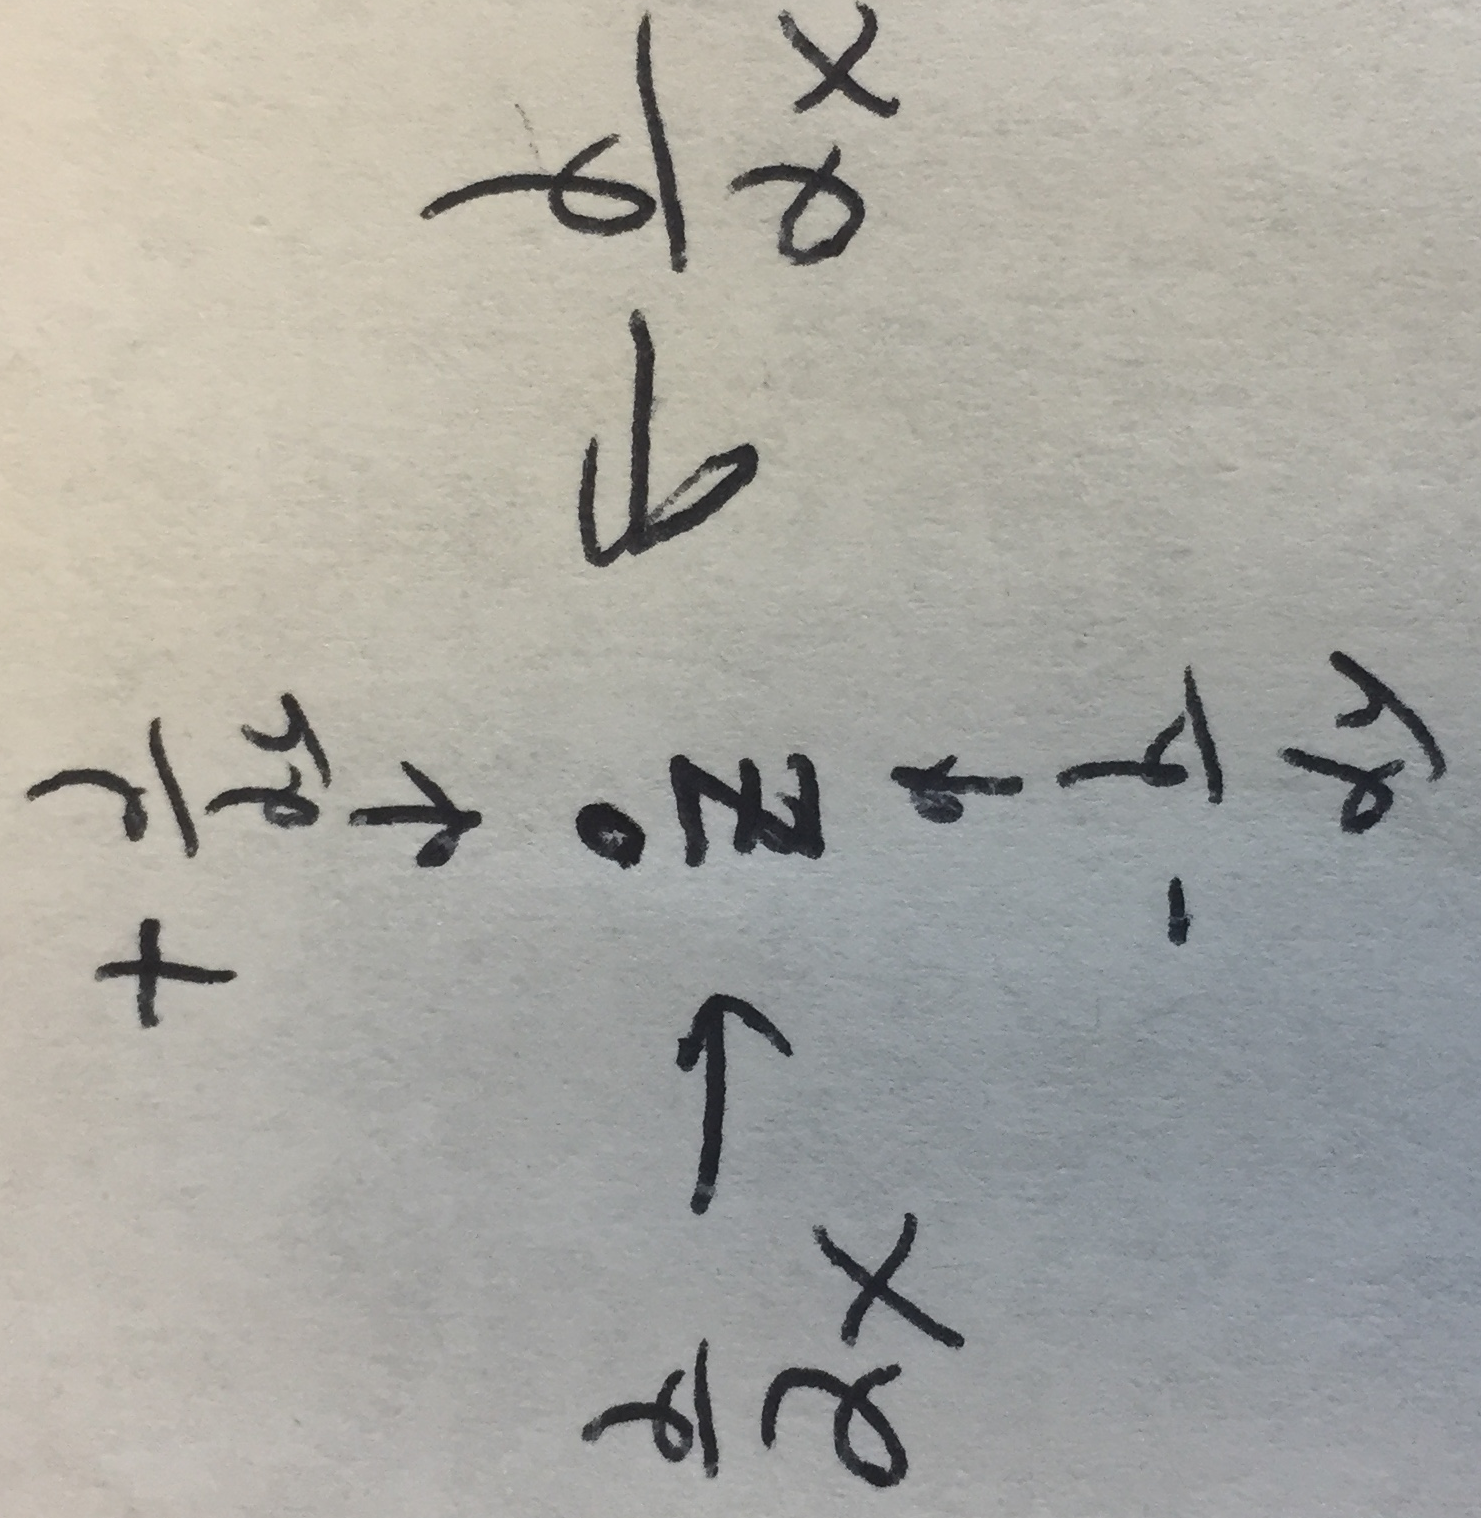
\includegraphics[scale=0.2]{Figures/approach.png}
    \caption{Make a caption different paths}
\end{figure}
The Cauchy-Riemann equations are derived from taking a  differential with respect to x and y  and then relating the Real part and imaginary part. Note: that for the imaginary piece we multiply by i thus getting a negative:
To be analytic we need 
\be
\frac{\pd f}{\pd x} = \frac{\pd f}{\pd y}
\ee
But in reality we have f=x+iy, therefore
\be
\begin{split}
    \frac{\pd f}{\pd x} &= \frac{1}{i}\frac{\pd}{\pd y}\\
    \frac{\partial f}{\partial x} &= \frac{\partial u}{\partial x}+ i\frac{\partial v}{\partial x}\\
    &= \frac{1}{i}\frac{\partial f}{\partial y}\\
    &= \frac{1}{i}\left[\frac{\partial u}{\partial y}+\frac{\partial v}{\partial y} i\right] \\
    &= \frac{1}{i}\left(\frac{\partial u}{\partial y}\right)+\frac{\partial v}{\partial y} i
\end{split}
\ee
This produces the Cauchy Riemann Equation
\be
\frac{\pd U}{\pd x} = \frac{\pd V}{\pd y}i\frac{\pd V}{\pd x} = -\frac{\pd U}{\pd y}
\ee
So an analytic function is a function that satifies the Cauchy Riemann Equation.
Not every function will satisfy this equation!

\subsubsection*{Analytic Example}
\be
\begin{split}
 f(z)=z^2 &= x^2 - y^2 + i(2xy) \\
 u &= x^2-y^2\\
 v &=2xy \\
 \frac{\partial u}{\partial x} &= 2x \frac{\partial v}{\partial y}\\
\frac{\partial v}{\partial x} &=2y = -\frac{\partial u}{\partial y}
\end{split}
\ee
z$^2$ is na example of an analytic function. 

\subsubsection*{Non-Analytic Example}
\be
\begin{split}
    f=z^*=x-iy  \\
\frac{\partial u}{\partial x} = 1 \neq \frac{\partial v}{\partial y} = -1
\end{split}
\ee

\subsection*{Line Integrals}
To compute a line integral we need to define the line, which sets our path. 
Therefore these calculations are path depedent, a different line computes a different value. 
So we cna compute an integral between 2 points z$_1$ and z$_2$ using the path L.
\begin{figure}[H]
  \centering
  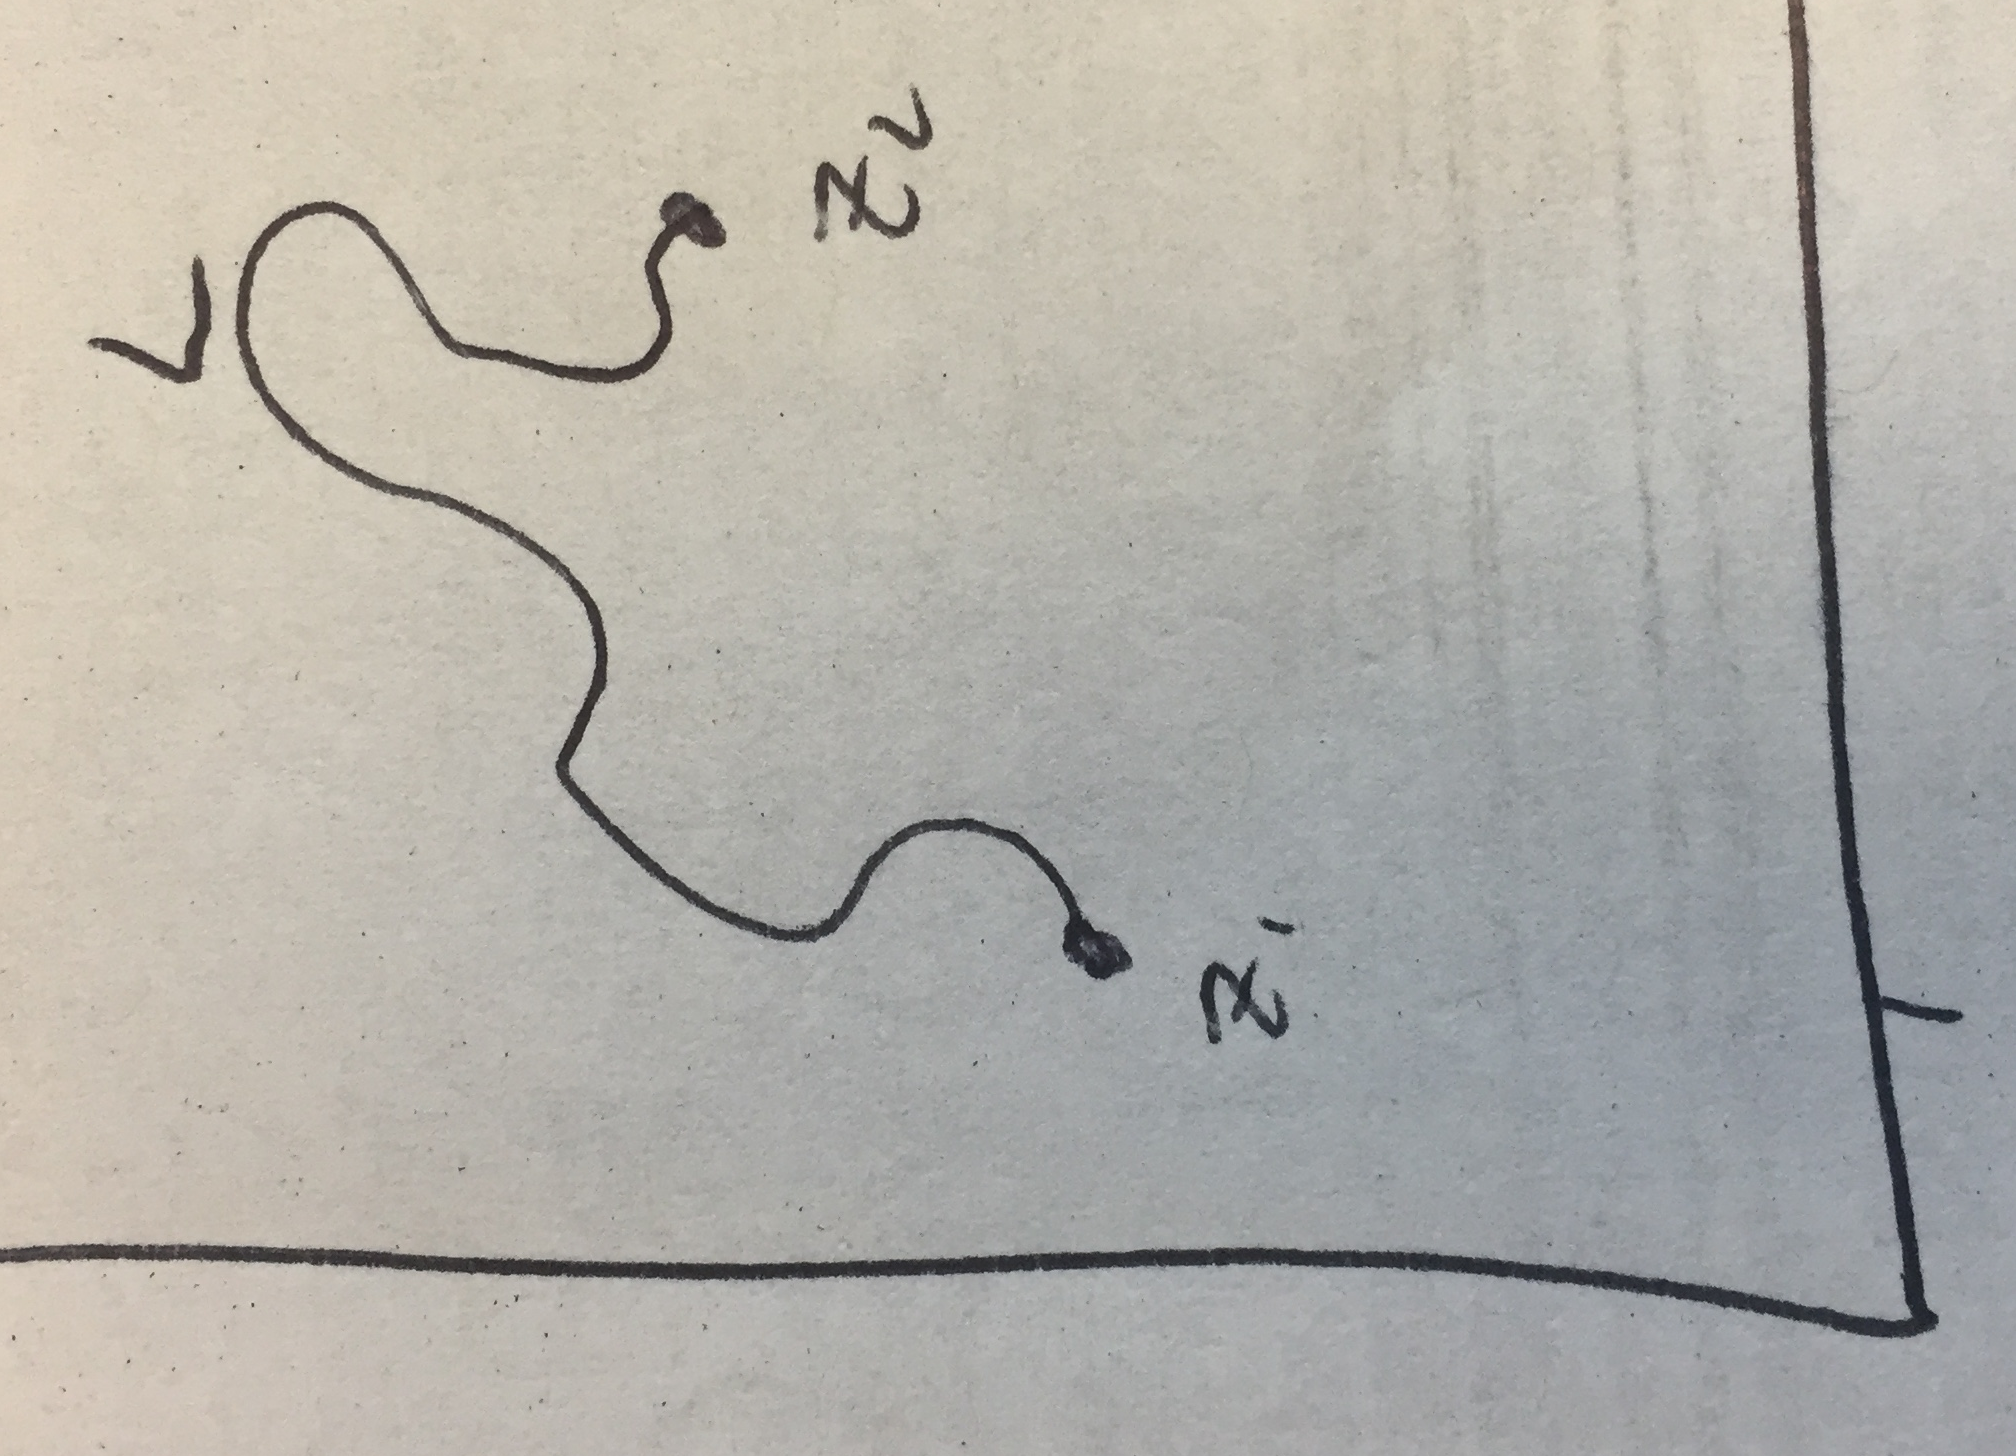
\includegraphics[scale=0.2]{Figures/line.png}
    \caption{Make a caption different points z and line L axis are x/y to give points z}
\end{figure}

The \textbf{Cauchy Theorem} states that such an integral is path independent if f(z) is regular in D $\epsilon$ L, in the domain containing L.  
\be
\int_{z_1}^{z_2} f(z) dz
\ee

Equivalently if an integral does not depend on its path, we can consider an integral over a closed contour C
\begin{figure}[H]
  \centering
    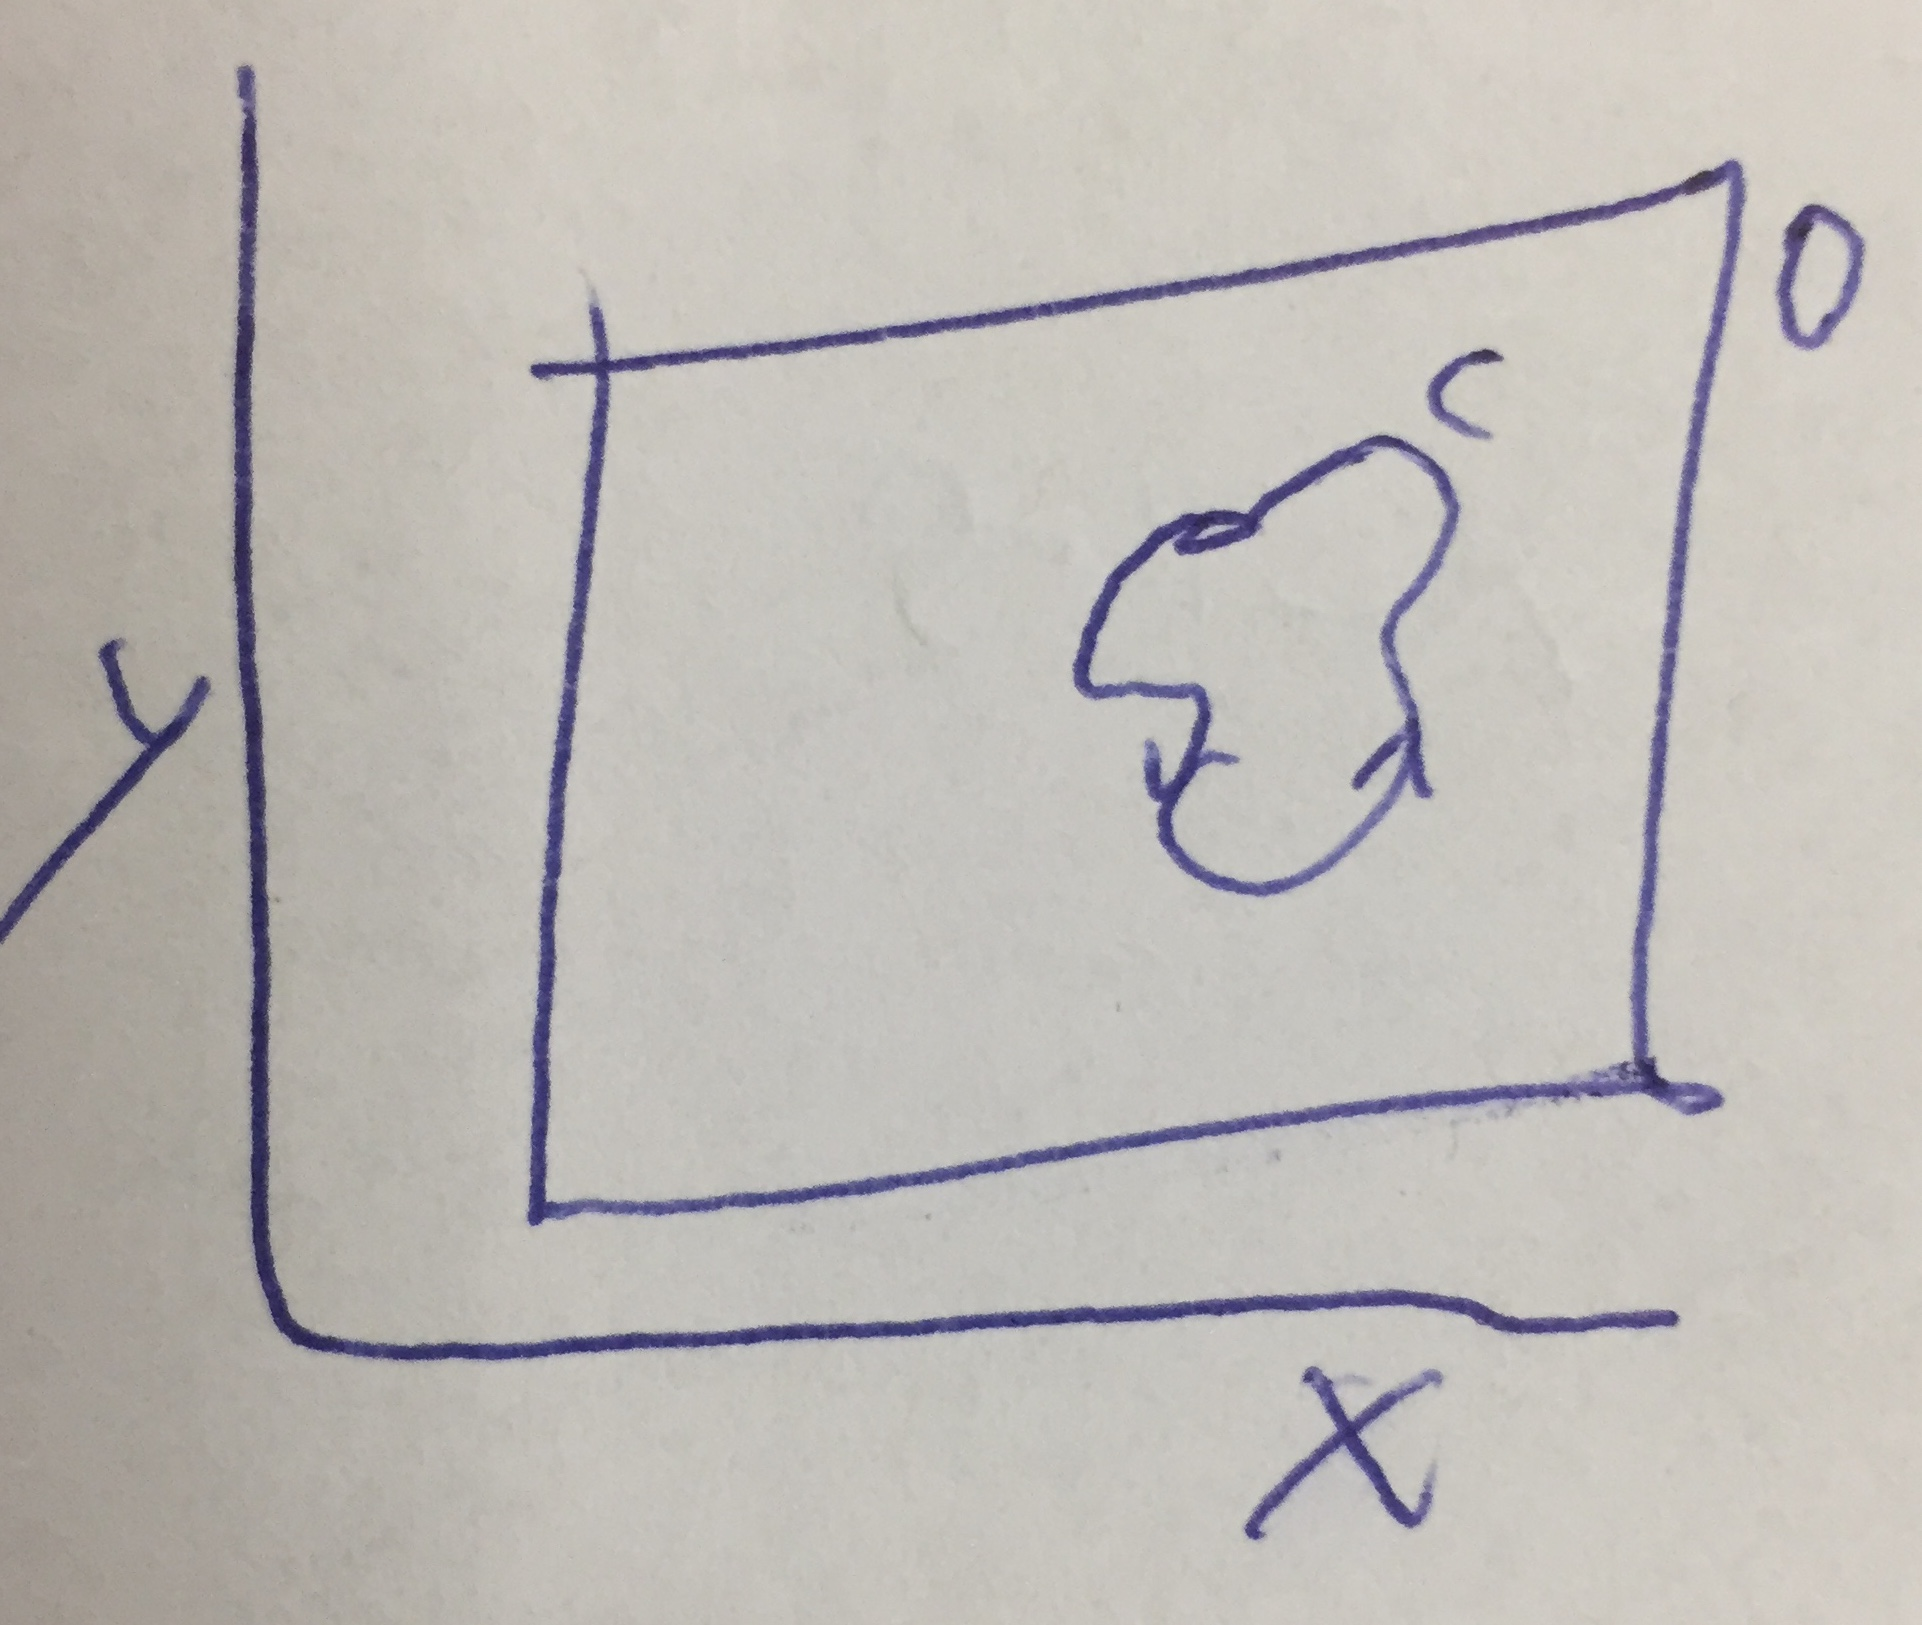
\includegraphics[scale=0.2]{Figures/contour.png}
    \caption{Make a caption different points z1,z2 and line L. Should be on xy coordinate axis and usrronided by a domain D. }
\end{figure}
If the integral is not path depedent, than our closed contour integral must evaluate to 0 (this statement is equivalent to the Cauchy theorem). 
\be
\oint\limits_{C \epsilon D} f(z) dz = 0
\ee

\subsection*{Complex Integration}
If f(x) is some function we are interested in integrating (assume it is analytic) we can instead compute the integral over f(z) to solve for f(x). 
This is a generalization of real calculus. 
\begin{figure}[H]
  \centering
    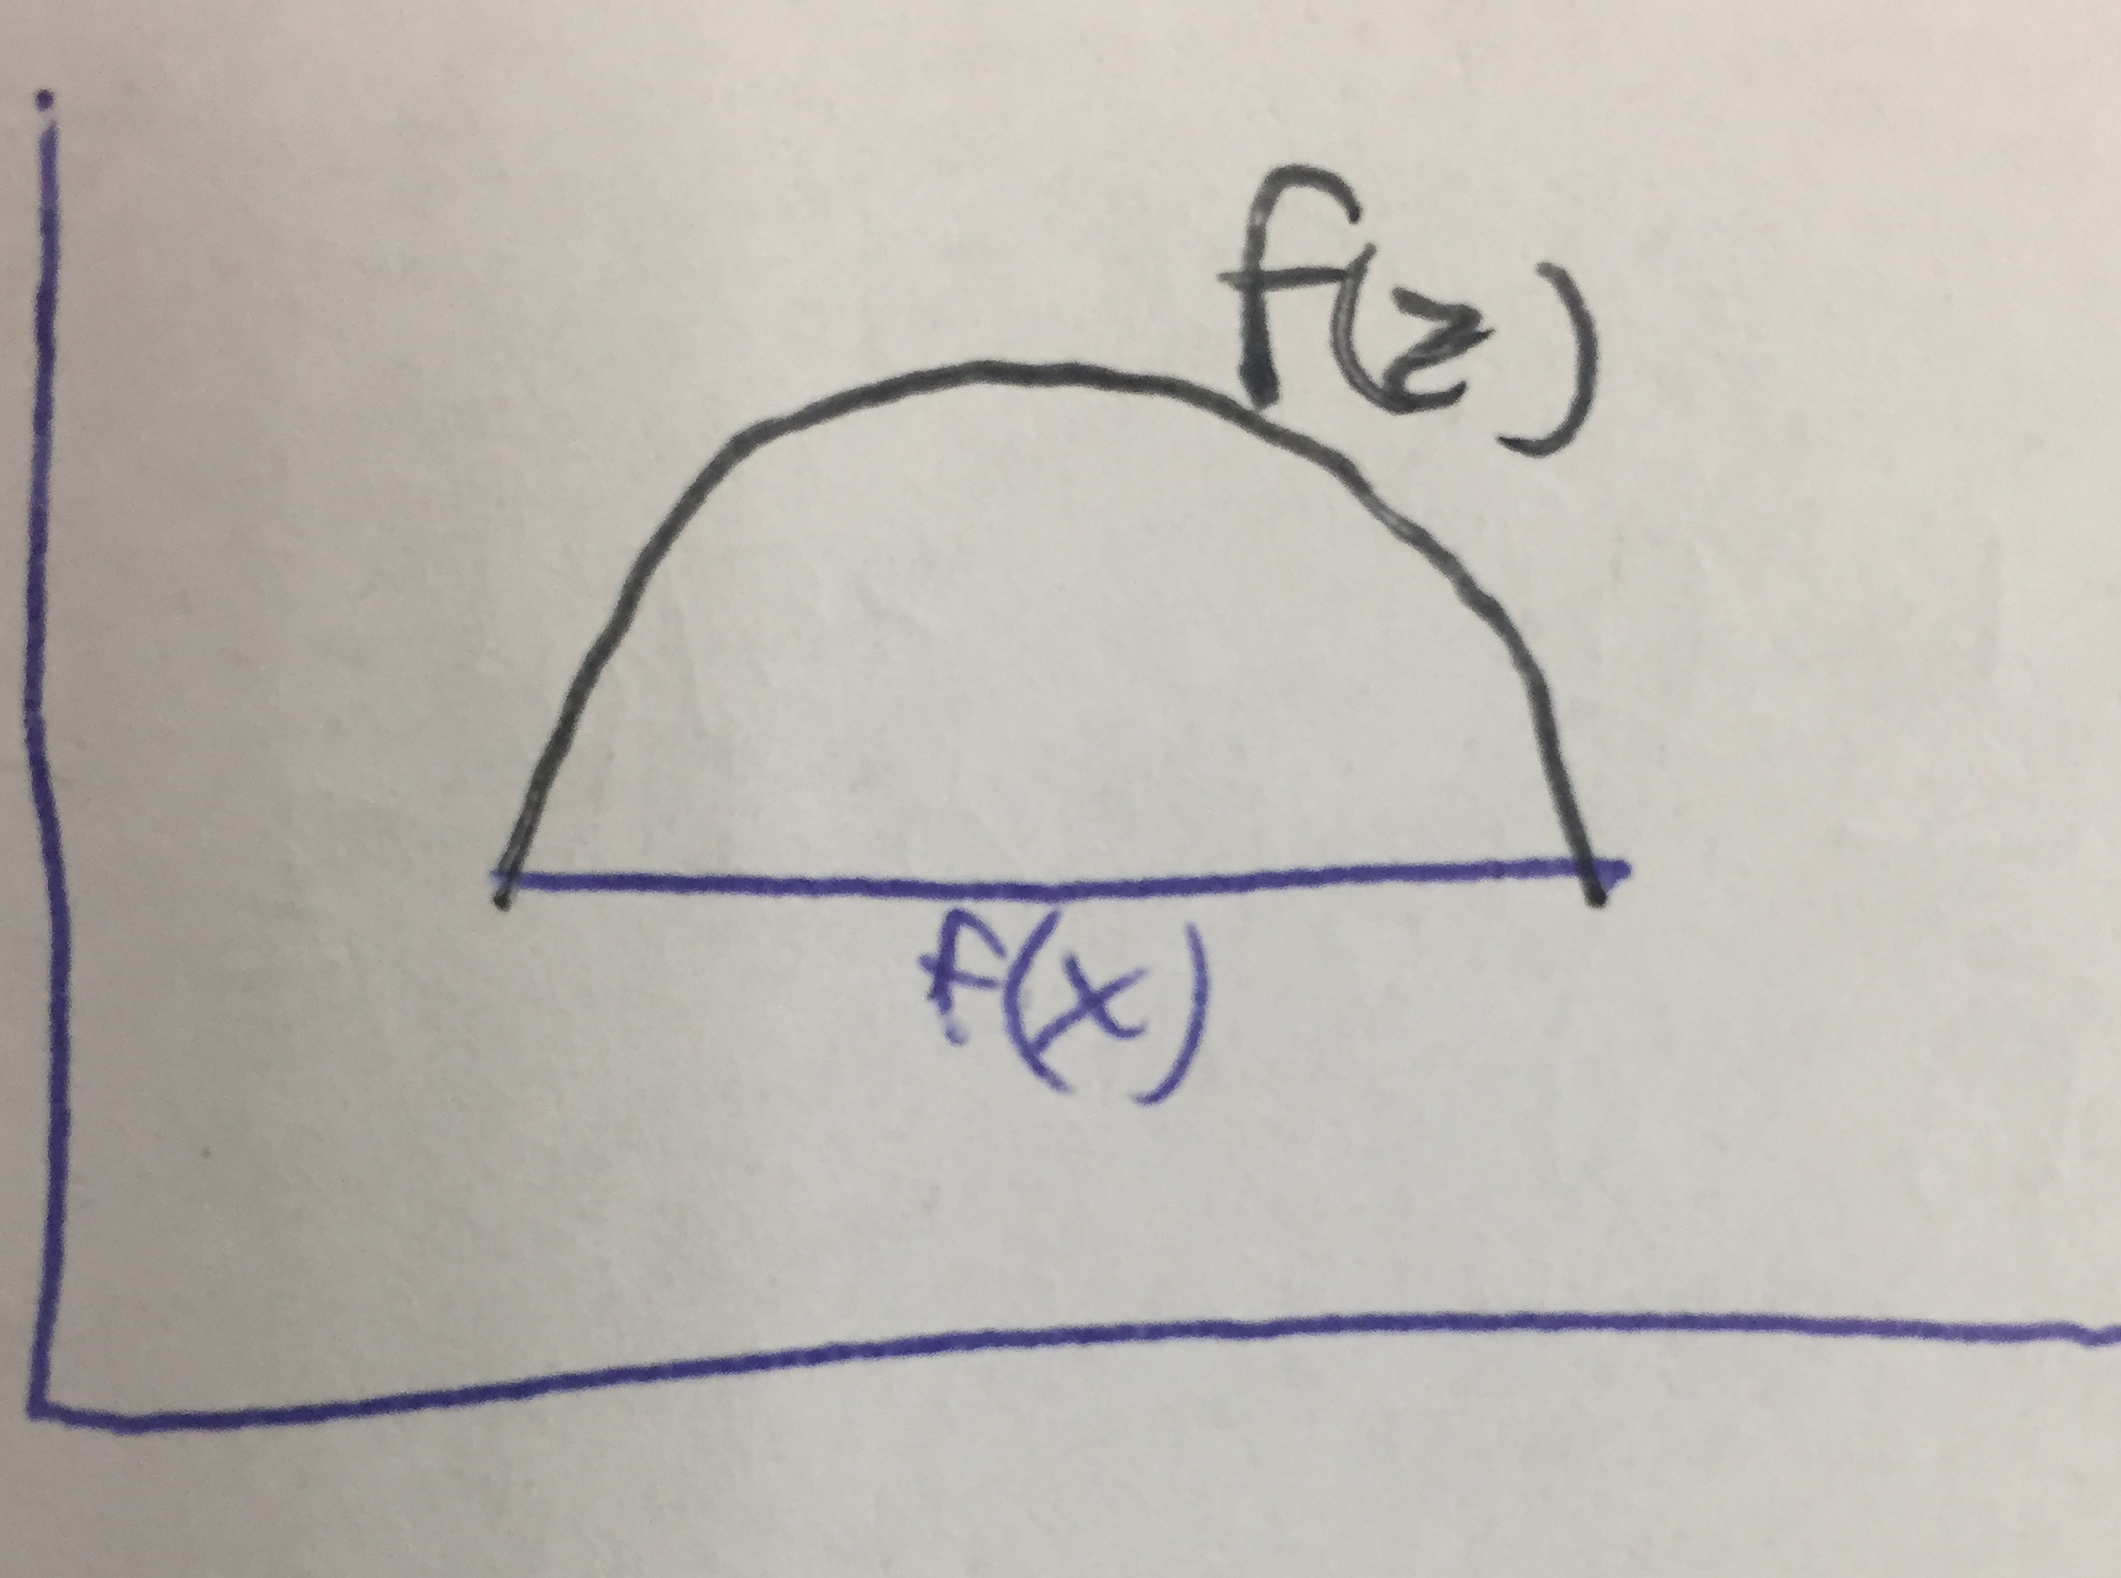
\includegraphics[scale=0.2]{Figures/motivation.png}
    \caption{Make a caption. compute real integral f(x) using complex contour f(z) and taking advantage of the cauchy theorem. }
\end{figure}

If F(z) is regular in D, than any $\frac{\pd^n}{\pd z^n}f(z)$ exists for all n, and the derivitive is a regular function in D.
Therfore if 1 derivitive exists, they all exist in D.

So a function that has a first derivitive in D, bu thigher orderderivitives do not exists, means the funciton is not analytic in D. 

\subsection*{Cauchy Integral Formula}
The Cauchy Integral Formula is over a closed contour
\be
f^{n}(z) = \frac{d^n f}{dz^n}  = \frac{n!}{2\pi i } \oint_\mathbb{C} \frac{f(w) dw}{(w-z)^{n+1}}
\ee
Where n is the order of your function.

It is convention for the contour to be traversed in a counter-clockwise fashion. 

% Need to add more context here










\end{document}
